%%
% This is an Overleaf template for presentations
% using the TUM Corporate Desing https://www.tum.de/cd
%
% For further details on how to use the template, take a look at our
% GitLab repository and browse through our test documents
% https://gitlab.lrz.de/latex4ei/tum-templates.
%
% The tumbeamer class is based on the beamer class.
% If you need further customization please consult the beamer class guide
% https://ctan.org/pkg/beamer.
% Additional class options are passed down to the base class.
%
% If you encounter any bugs or undesired behaviour, please raise an issue
% in our GitLab repository
% https://gitlab.lrz.de/latex4ei/tum-templates/issues
% and provide a description and minimal working example of your problem.
%%

\PassOptionsToClass{onlytextwidth}{beamer}

\documentclass[
  german,            % define the document language (english, german)
  aspectratio=169,    % define the aspect ratio (169, 43)
  % handout=2on1,       % create handout with multiple slides (2on1, 4on1)
  % partpage=false,     % insert page at beginning of parts (true, false)
  % sectionpage=true,   % insert page at beginning of sections (true, false)
]{tumbeamer}


% load additional packages
\usepackage{booktabs}
\usepackage{graphicx}
\usepackage{tikz}
\usepackage{url}
\usepackage{pgfplots}
\usepackage{hyperref}
\usepackage{pmboxdraw}
\usepackage{float}
\usepackage{babel}[ngerman]
\usepackage{csquotes}[autostyle]
\usepackage[useregional]{datetime2}

% tikz  
\usetikzlibrary{fit}

% image path
\graphicspath{ {./resources/} }

% presentation metadata
\title{Übung 02: RISC-V Assembly}
\subtitle{Einführung in die Rechnerarchitektur}
\author{Niklas Ladurner}

\institute{\theChairName\\\theDepartmentName\\\theUniversityName}
\date{\DTMdisplaydate{2024}{10}{25}{-1}}

\footline{\insertauthor~|~\insertshorttitle~|~\insertshortdate}


% macro to configure the style of the presentation
\TUMbeamersetup{
  title page = TUM tower,         % style of the title page
  part page = TUM toc,            % style of part pages
  section page = TUM toc,         % style of section pages
  content page = TUM more space,  % style of normal content pages
  tower scale = 1.0,              % scaling factor of TUM tower (if used)
  headline = TUM threeliner,      % which variation of headline to use
  footline = TUM default,         % which variation of footline to use
  % configure on which pages headlines and footlines should be printed
  headline on = {title page},
  footline on = {every page, title page=false},
}

% available frame styles for title page, part page, and section page:
% TUM default, TUM tower, TUM centered,
% TUM blue default, TUM blue tower, TUM blue centered,
% TUM shaded default, TUM shaded tower, TUM shaded centered,
% TUM flags
%
% additional frame styles for part page and section page:
% TUM toc
%
% available frame styles for content pages:
% TUM default, TUM more space
%
% available headline options:
% TUM empty, TUM oneliner, TUM twoliner, TUM threeliner, TUM logothreeliner
%
% available footline options:
% TUM empty, TUM default, TUM infoline


\begin{document}

\maketitle

\begin{frame}[c]{}{}
  \begin{center}
    \LARGE  Keine Garantie für die Richtigkeit der Tutorfolien.

    \Large Bei Unklarheiten/Unstimmigkeiten haben VL/ZÜ-Folien recht!
  \end{center}
\end{frame}

\begin{frame}[c]{Abstraktionsebenen}{}
  \begin{columns}[c]
    \begin{column}{0.6\textwidth}
      \begin{itemize}
        \item Code in einer Hochsprache (C, Java, \textellipsis) ist lediglich eine Abstraktion
        \item Compiler: Hochsprache $\rightarrow$ Assemblersprache
        \item Assembler: Assemblercode $\rightarrow$ Maschinensprache (1:1 Übersetzung)
        \item Maschinensprache ist plattformspezifisch!
        \item ISA: \enquote{Bedienungsanleitung} einer CPU
        \item RISC vs. CISC
      \end{itemize}
    \end{column}
    \begin{column}{0.3\textwidth}
      \begin{figure}
      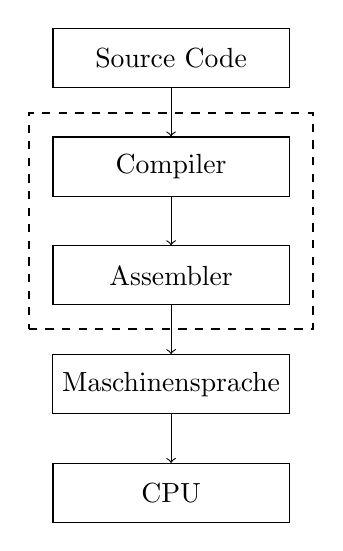
\begin{tikzpicture}[
          block/.style = {draw, rectangle, minimum width=3cm, minimum height=0.75cm, align=center},
          node distance=1.2cm
        ]

        \node[block] (source) at (0,0) {Source Code};
        \node[block, yshift=-1cm] (compiler)  at (source.south){Compiler};
        \node[block, yshift=-1cm] (assembler) at (compiler.south){Assembler};
        \node[block, yshift=-1cm] (machine) at (assembler.south) {Maschinensprache};
        \node[block, yshift=-1cm] (cpu) at (machine.south) {CPU};

        \draw[->] (source) -- (compiler) node[midway, right] {};
        \draw[->] (compiler) -- (assembler) node[midway, right] {};
        \draw[->] (assembler) -- (machine) node[midway, right] {};
        \draw[->] (machine) -- (cpu) node[midway, right] {};

        \node[draw, dashed, thick, inner sep=0.3cm, fit=(compiler) (assembler)] {};
      \end{tikzpicture}
      \footnotesize  (Abbildung stark vereinfacht)
    \end{figure}
    \end{column}
  \end{columns}
\end{frame}

\begin{frame}[c]{RISC-V}{}
  \begin{columns}[c]
    \begin{column}{0.6\textwidth}
      \begin{itemize}
        \item eine von vielen Assemblersprachen
        \item Datenwortbreite: 32 Bit (4 Byte)
        \item Little-Endian-Architektur
        \item 32 Register, einige davon mit spezieller Funktion
        \item grundlegende Instruktionen auf 32 Bit begrenzt 
        $\rightarrow$ Konstanten müssen zusammengebastelt werden
        \item Immediates sind 12 Bit lang (sign-extended)
      \end{itemize}
    \end{column}
    \begin{column}{0.3\textwidth}
      
\includegraphics[width=\linewidth]{risc_v_logo.png}
    \end{column}
  \end{columns}
\end{frame}

\begin{frame}[c]{}{}
  \begin{center}
    \LARGE Fragen?
  \end{center}
\end{frame}


\begin{frame}[c]{Artemis-Hausaufgaben}{}
  \begin{itemize}
    \item \enquote{H02 --- Festkommarechnung} bis 03.11.2024 23:59 Uhr
    \item Vorüberlegungen zu Festkommarechnung auf Mitschrift WS 23/24
  \end{itemize}
\end{frame}

\begin{frame}[fragile, c]{Links}{}
  \begin{itemize}
    \item Zulip: \href{https://zulip.in.tum.de/#narrow/stream/2661-ERA-Tutorium---Do-1600-1}{\enquote{ERA Tutorium - Do-1600-1}}
          bzw. \href{https://zulip.in.tum.de/#narrow/stream/2675-ERA-Tutorium---Fr-1500-2 }{\enquote{ERA Tutorium - Fr-1500-2}}
    \item \href{https://www.moodle.tum.de/course/view.php?id=100633}{ERA-Moodle-Kurs}
    \item \href{https://artemis.in.tum.de/courses/401}{ERA-Artemis-Kurs}
    \item \href{https://vanhunteradams.com/FixedPoint/FixedPoint.html}{Einführung Fixpunktarithmetik}, \href{https://specbranch.com/posts/fixed-point/}{Alternative}
    \item \href{https://msyksphinz-self.github.io/riscv-isadoc/html/index.html}{Übersicht an RISC-V-Instruktionen}
  \end{itemize}
\end{frame}

\maketitle

\end{document}
